
\documentclass{article}
\usepackage{ stmaryrd }
\usepackage{amsmath,amsthm,amsfonts,amssymb,array}


\usepackage{geometry}
\usepackage{todonotes}



\usepackage[center,xpart]{figbib}
\usepackage{hyperref}
\geometry{verbose,tmargin=2cm,bmargin=2cm,lmargin=2cm,rmargin=2cm}
\usepackage[section]{placeins}
\usepackage{caption}
\usepackage{xcolor}

\newcommand{\etodo}[1]{\textcolor{purple}{[E: #1]}}
\newtheorem{theorem}{Theorem}[section]
\numberwithin{theorem}{subsection}
\newtheorem{claim}[theorem]{Claim}
\newtheorem{corollary}[theorem]{Corollary}
\newtheorem*{definition}{Definition}
\newtheorem{lemma}[theorem]{Lemma}
\newtheorem{exercise}[theorem]{Excercise}
\newtheorem{remark}[theorem]{Remark}
\theoremstyle{remark}
\newtheorem*{solution}{Solution}

\newcommand{\eqdef}{=\mathrel{\mathop:}}

\begin{document}

\title{Problem Space formulation}
\date{\vspace{-5ex}}
\maketitle

\section{Introduction}

The following is an explanation of the formal terms used in defining
and identifiying the cuts used to generate the plots for re-compare library.

\begin{definition}[Solution]
	Given a general problem $F$ which is takes parameters $p_{i}\in P_{i}\mid1\le i\le n$
	and whose possible solution can be represented in a tuple of independant
	values $s_{i}\in S_{i}\mid1\le j\le m$, the problem can be seen as
	a function
	\[\begin{array}{l}
	f:P\rightarrow 2^{S} \\
	P=\times_{i=1}^nP_i\\
	S=\times_{j=1}^mS_i \\
	\end{array}
	\]
	we would say that $s\in S$ is a solution of $p\in P$ if $s\in f(p)$.
\end{definition}

\begin{definition}[Problem space]
	Using the notations above, we mark $ P $ as the parameter space, $ S $ as the solution space and $ Pr \eqdef P \times S  $ as the solution space. We define $ \{ (p,s)) \mid p\in P, s\inf(p) \} $ as the proper (feasible) problem space
\end{definition}

When analyzing high dimensional information, we often time try look for a dependancy between some $ P_i $ and some $ S_j $ when leaving all other $ P_k \mid k\ne i $ constants. This defines a sub space on the problem space.

\begin{definition}[Cuts]
	A cut of the problem space of a problem $ f $ is a sub space the proper solution space
	\[ \pi_{k_1=c_1,\dots,k_r=c_r,k'_1=d_1,\dots,k'_{r'}=d_r' }(Pr) = \{ (p,f(p)) \mid p_{k_i}=c_i, s_{k'_j}=d_j \} \]
	Basically, we take only the proper tuples that agreed with the designated constant equality constraints we put on some of the dimensions of the problem space.

	We define a $ k $-cut as a cut that is not constrained on $ k $ dimensions. We define a $ r_1,r_2 $-cut as a subspace that in not constrained only on dimensions $ r_1 $ and $ r_2 $. This definition generalises to any amount of dimensions.
\end{definition}


\section*{Analyzing and Visualizing }

When trying to analyze a Problem space by experimental computations and present results in a manner
that's is informative for a human, we will present 3 dimensional cuts of the problems space as 2 dimensional plots as \textbf{discrete layer plots}.

\begin{definition}[DLPs (Discrete layer plots) ]
	A DLP is a tuple of the form $ (Q_{1},Q_{2},F,C_1,C_2) $ Where
	\begin{itemize}
		\item $ Q_1, Q_2, F $ are dimensions of the problem space.
		\item $ C_1,C_2 $ are discrete subsets of $ Q_1,Q_2 $ respectively.
	\end{itemize}
\end{definition}


We visualize the DLP on a $ 2 $-dimensional plot by taking
\begin{itemize}
	\item $ Q_1 $ to be the independent variable on the $ x $ axis
	\item $ F $ to be the dependent variable on the $ y $ axis
	\item $ Q_2 $ to be another independent variable that varies across layers of the plot
\end{itemize}
The discreteness restriction on $ Q_2 $ stems from a visualization constraint (since we cant have a continuum of layers in a plot) and both independent parameters are constrained because we are sampling Algorithms on finite sets of inputs.


\subsection*{Localization to Re-comp}

In Re-comp we compare algorithms of the type $match(text,patern)$ and are usually interested in the time performance of the matching operations. Thus, for a set of Algs $A$ and a space of texts and regex patterns $T,R$ we would define the Problem space as
\[\begin{array}{l}
P=A\times T\times R \\
S=\mathbb{R}\cong time \\
\end{array}
\]

Since we are interested in seeing how different algorithms fair in time across varying texts and patterns, we are
interested in DLPs of the form $(T_{i},A,time,C,A)$ or $(R_{i},A,time,C,A)$.
This basically means that we show all the results in terms of $ time $ keeping all parameters of the problems constant except the algorithm chosen and a single parameter of the regex's or texts.

\begin{figure}[h]
	\centering
	\captionsetup{justification=centering,width=0.5\textwidth}
	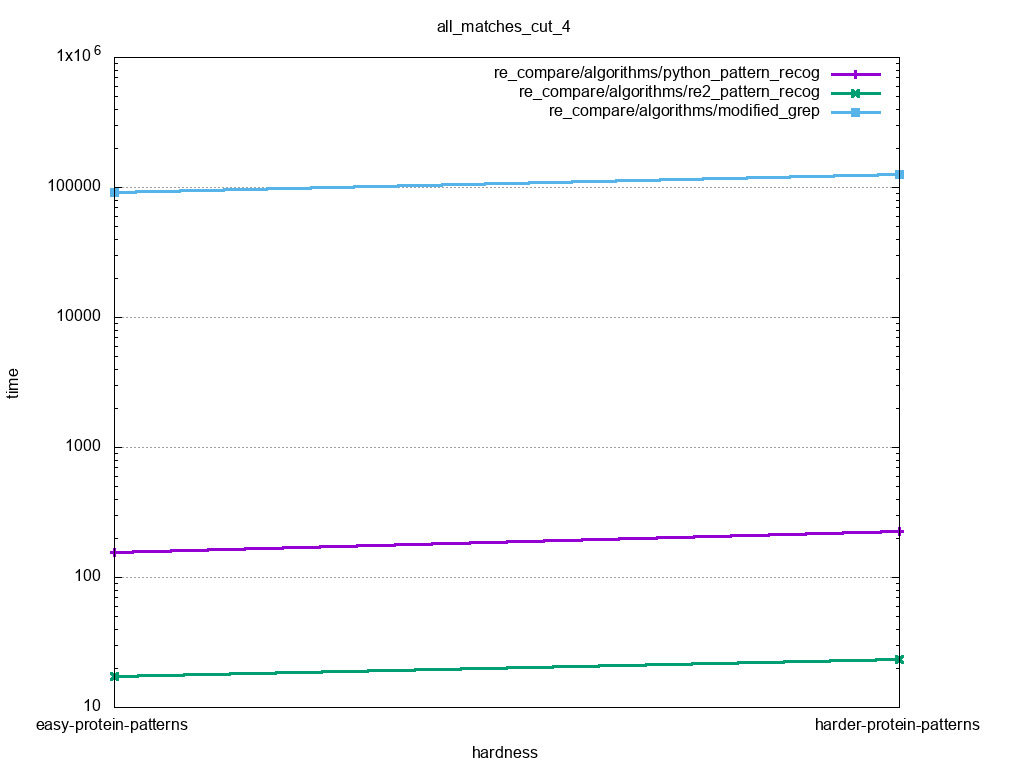
\includegraphics[width=0.5\textwidth]{../output/all_matches_cut_4.png}
  \caption{An example of DLP plot from re-compare. $R_i$ is regex difficulty with $C$ being \{easy,hard\}. $A$ consists of $3$ regex matching Algs, each of which gets a label }
	\label{fig:medial}
\end{figure}

What makes re-compare stands out is that it computes all such DLPs given any parametrisation to the regex space and text space.

\end{document}
